\documentclass[10pt, compress]{beamer}
\usetheme{m}
\usepackage{multimedia}
 
 \usepackage{booktabs} % for better tables
 \usepackage{natbib}  % for better citations
 \usepackage{media9} % for includemedia i.e. videos
 \usepackage{xcolor} % for more colors
 
\usepackage{tikz}
\usetikzlibrary{shadows,trees}
\usetikzlibrary{shapes,calc,backgrounds}
\usetikzlibrary{fadings}
\usetikzlibrary{arrows}
\usetikzlibrary{fit,positioning}
\usepackage{environ}
\makeatletter
\newsavebox{\measure@tikzpicture}
\NewEnviron{scaletikzpicturetowidth}[1]{%
  \def\tikz@width{#1}%
  \def\tikzscale{1}\begin{lrbox}{\measure@tikzpicture}%
  \BODY
  \end{lrbox}%
  \pgfmathparse{#1/\wd\measure@tikzpicture}%
  \edef\tikzscale{\pgfmathresult}%
  \BODY
}
\makeatother
%\usepgfplotslibrary{dateplot,calc}

\usepackage{graphicx}
\usepackage{url}
\usepackage{caption}
\usepackage{amssymb}
\usepackage{amsmath}
\usepackage{multirow}
\usepackage[position=bottom,labelfont=bf,textfont={sl,bf}]{subfig}
\usepackage[utf8]{inputenc}
\usepackage{relsize}

\usepackage{epsfig}
\usepackage[]{algorithm2e}
%
\title{Motion and Observation Models for Behavior Understanding}
\author{Suren Kumar \\ Research Fellow \\ Electrical Engineering and Computer
Science}
\institute{University of Michigan, Ann Arbor}
\date{\today}

\begin{document}

\maketitle
% Introduction
%\include{intro}
% Tracking
%\include{tracking}
% Pose Estimation

\section[Pose Estimation]{Model-less Pose Estimation}
\begin{frame}{Problem Statement}
\begin{figure}
\centering
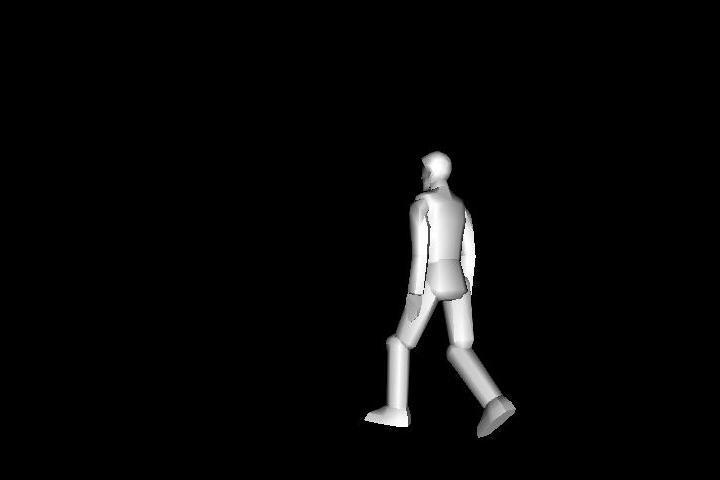
\includegraphics[height=0.6\linewidth,trim = 60mm 5mm 35mm 20mm,clip]{figures/human_figure3d}
\end{figure}
\end{frame}

\begin{frame}{Parts of Pose Estimator}
\begin{itemize}
\item Motion Model : Second Order motion continuity
\item Observation Model : Mapping features to pose using Gaussian Processes
\item Estimation : Kalman Filter
\end{itemize}
\end{frame}

\begin{frame}{Previous Work }
  \begin{columns}
    \begin{column}{0.5\textwidth}
Model Based Optimization [Agarwal et. al, RSS 2012]:
      \centering
      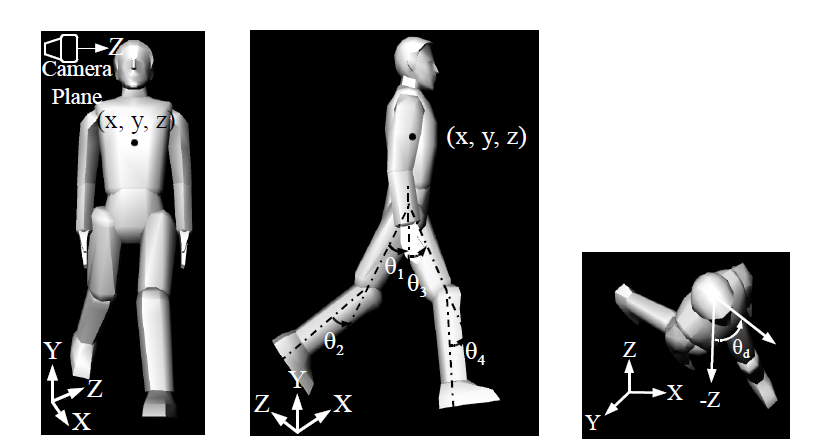
\includegraphics[width=1\textwidth]{figures/person_model}
\begin{itemize}
\item Computationally expensive
\item Model Required: Articulation, CAD
\item Often requires background subtraction
\end{itemize}
    \end{column}
\begin{column}{0.5\textwidth}
Template Based Methods  [Reiter et. al, CARS 2012]
  \begin{columns}
    \begin{column}{0.3\textwidth}
      \centering
      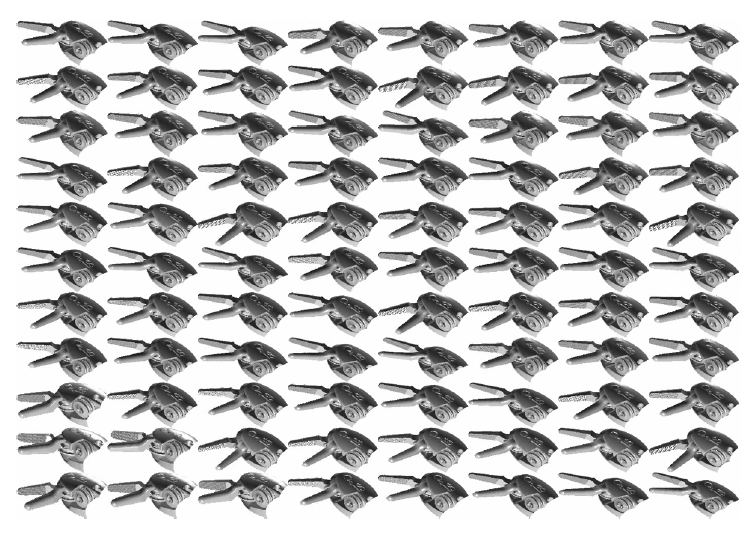
\includegraphics[width=1\textwidth]{figures/tool_model}
    \end{column}
    \begin{column}{0.7\textwidth}
      \centering
      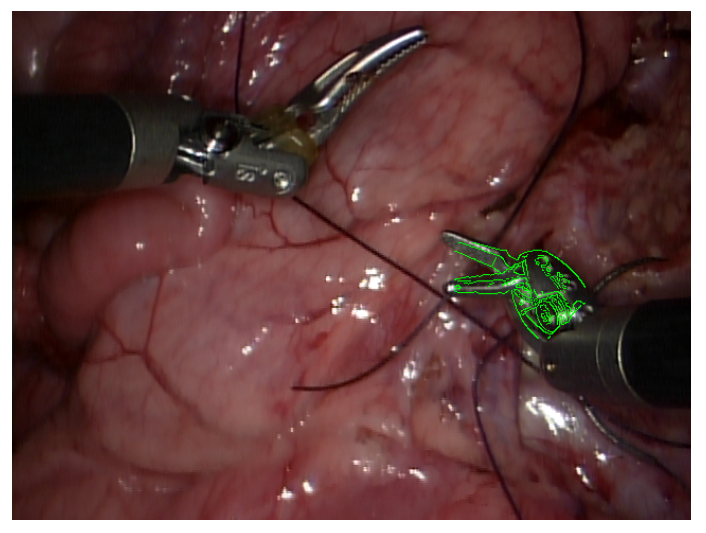
\includegraphics[width = 1\textwidth]{figures/tool_image}
    \end{column}
  \end{columns}
\begin{itemize}
\item Curse of Dimensionality
\item Model Required: Articulation, CAD, Visual
\end{itemize}
\end{column}
  \end{columns}
\end{frame}

\subsection[]{GPR Pose Estimation}
\begin{frame}{Model-less Pose Estimation}
\begin{block}{Guiding Principles}
\begin{itemize}
\item Real-time performance
\item Measure of confidence in estimates
\end{itemize}
\end{block}

\begin{figure}
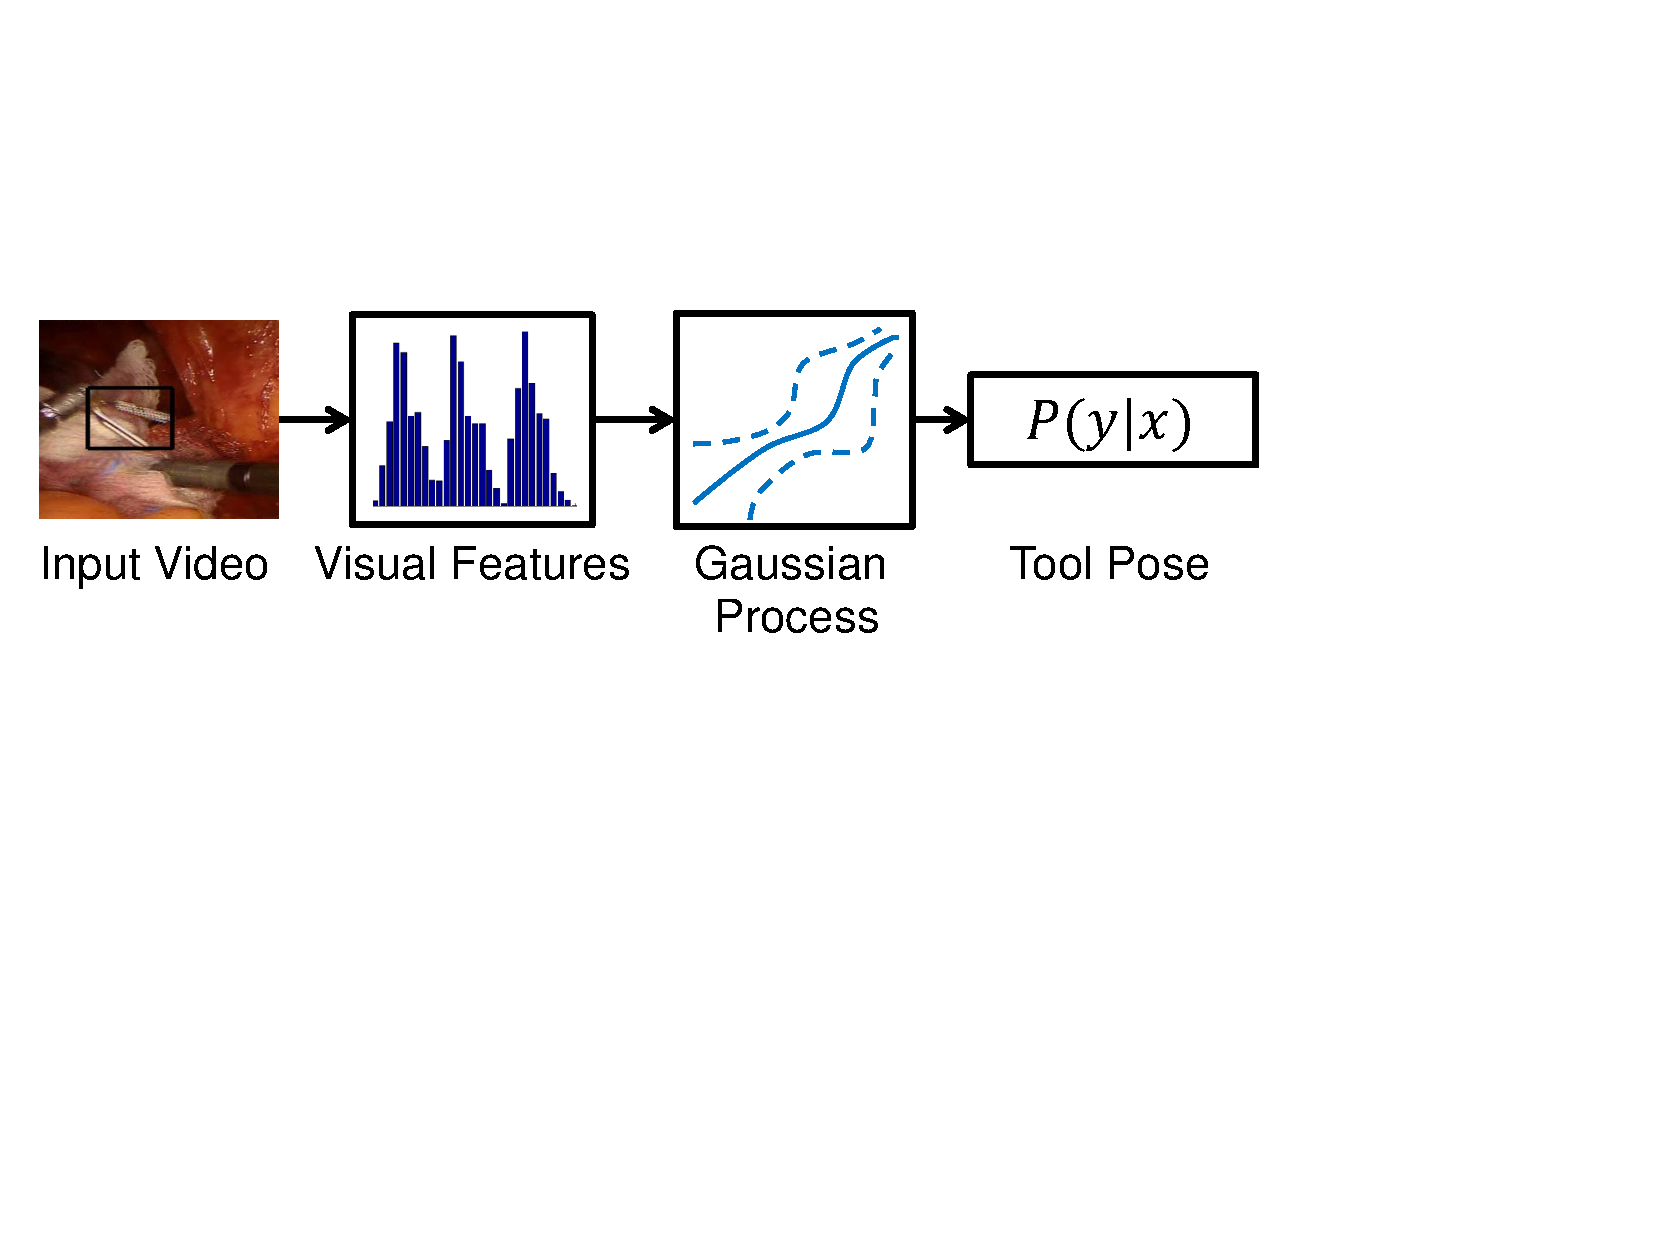
\includegraphics[scale=0.5,trim=5mm 100mm 60mm 50mm,clip]{figures/surgical/flow_chart}
\end{figure}

\begin{itemize}
%\item Requires ground truth poses for generalization
\item Model Required: Articulation
\item Map generic visual features $x$ to tool end-effector pose estimate $y$
\item Tool Pose $y$ represents orientation, end-effector opening angle
\end{itemize}

\end{frame}


\begin{frame}{Gaussian Process Regression}
\begin{block}{Problem with Regression Models}
\begin{itemize}
\item Parametric Models
\item Prediction is dependent on the chosen model
\end{itemize}
\end{block}
%Gaussian process regression essentially defines a distribution over function with inference taking place in the space of functions, thus avoiding the need to estimate the weights/parameters associated with traditional regression methods.
\begin{block}{Gaussian Process Regression}
$f(x) \sim \mathbb{GP}(m(x),k(x,x^1))$
\begin{itemize}
\item Inference takes place in space of functions
\item Makes minimal assumptions on the underlying data distribution
\item High variance in regions with sparse ground truth data
\end{itemize}
\end{block}
\end{frame}

\begin{frame}{Gaussian Process Regression}
$f(x): x \mapsto y$. 
\begin{itemize}
\item Input: Ground truth data  from $(\mathbf{X},\mathbf{y})$ from $n$ observations
\item Output: Pose $y*$ for a new image with associated feature vector $x^*$, $p(y^*|x^*)$. 
\item Measurement Process: $y = f(x)+\epsilon $, $\epsilon \sim \mathcal{N}(0,\sigma^2)$
\end{itemize}
Inference:
\begin{itemize}
\item $f(x) \sim \mathbb{GP}(m(x),k(x,x^1))$
\item $\mathrm{cov}(f(x_p),f(x_q)) = k(x_p,x_q) = \exp^{-\frac{1}{2l}(x_p-x_q)^2}$
\item For two observation, $y_p,y_q$, we get, $\mathrm{cov}(y_p,y_q)=k(x_p,x_q)+\sigma^{2}\delta_{pq} $
\end{itemize}
Prediction: Marginalize training data,
\begin{align}
\mathbf{f}^*|\mathbf{X},\mathbf{y},X^*&\sim \mathcal{N}(\mathbf{\bar{f}}^*,\mathrm{cov}(\mathbf{f}^*)) \label{eq:final_prediction}\\
\mathbf{\bar{f}}^* = &K(X^*,X)[K(X,X)+\sigma^2I]^{-1}\mathbf{y} \nonumber \\
\mathrm{cov}(\mathbf{f}^*) = &K(X^*,X^*)- K(X^*,X)[K(X,X)+\sigma^2I]^{-1}K(X,X^*) \nonumber 
\end{align}
%Intuitively this algorithm gives high confidence estimates in the region of feature space with lot of ground truth data, and estimates with high variance in regions with sparse ground truth data. 
\end{frame}

\subsection[]{Smoothing Predictions}
\begin{frame}{Improving Prediction}
\begin{itemize}
\item Regression process predicts pose solely using one image
 \item Smoothness in surgical actions
\end{itemize}

\begin{block}{Motion Continuity}
 Consider a single $k^{th}$ element of the pose state $y(k)$, 
\begin{align}
\begin{bmatrix}
y(k)_{t}\\
\dot{y}(k)_{t}
\end{bmatrix}=
\begin{bmatrix}
1 & \delta t\\
0 & 1
\end{bmatrix}\begin{bmatrix}
y(k)_{t-1}\\
\dot{y}(k)_{t-1}
\end{bmatrix}+
\begin{bmatrix}
\frac{1}{2} \delta t^2 \\
\delta t
\end{bmatrix}\ddot{y}(k)_{t-1} \label{eq:state_prop}
\end{align}
Acceleration is modeled as zero mean Gaussian white noise $\ddot{y}(k)_t \sim \mathcal{N}(0,\sigma_a^2) \forall t $.
\end{block}
\end{frame}

\begin{frame}{Improving Predictions}
The observation model is the Gaussian process regression framework which can be represented by 
\begin{align}
z_t = \begin{bmatrix}
1&0
\end{bmatrix}\begin{bmatrix}
y(k)_{t}\\
\dot{y}(k)_{t}
\end{bmatrix}+v_t \label{eq:state_obs}
\end{align}
\begin{figure}
\centering
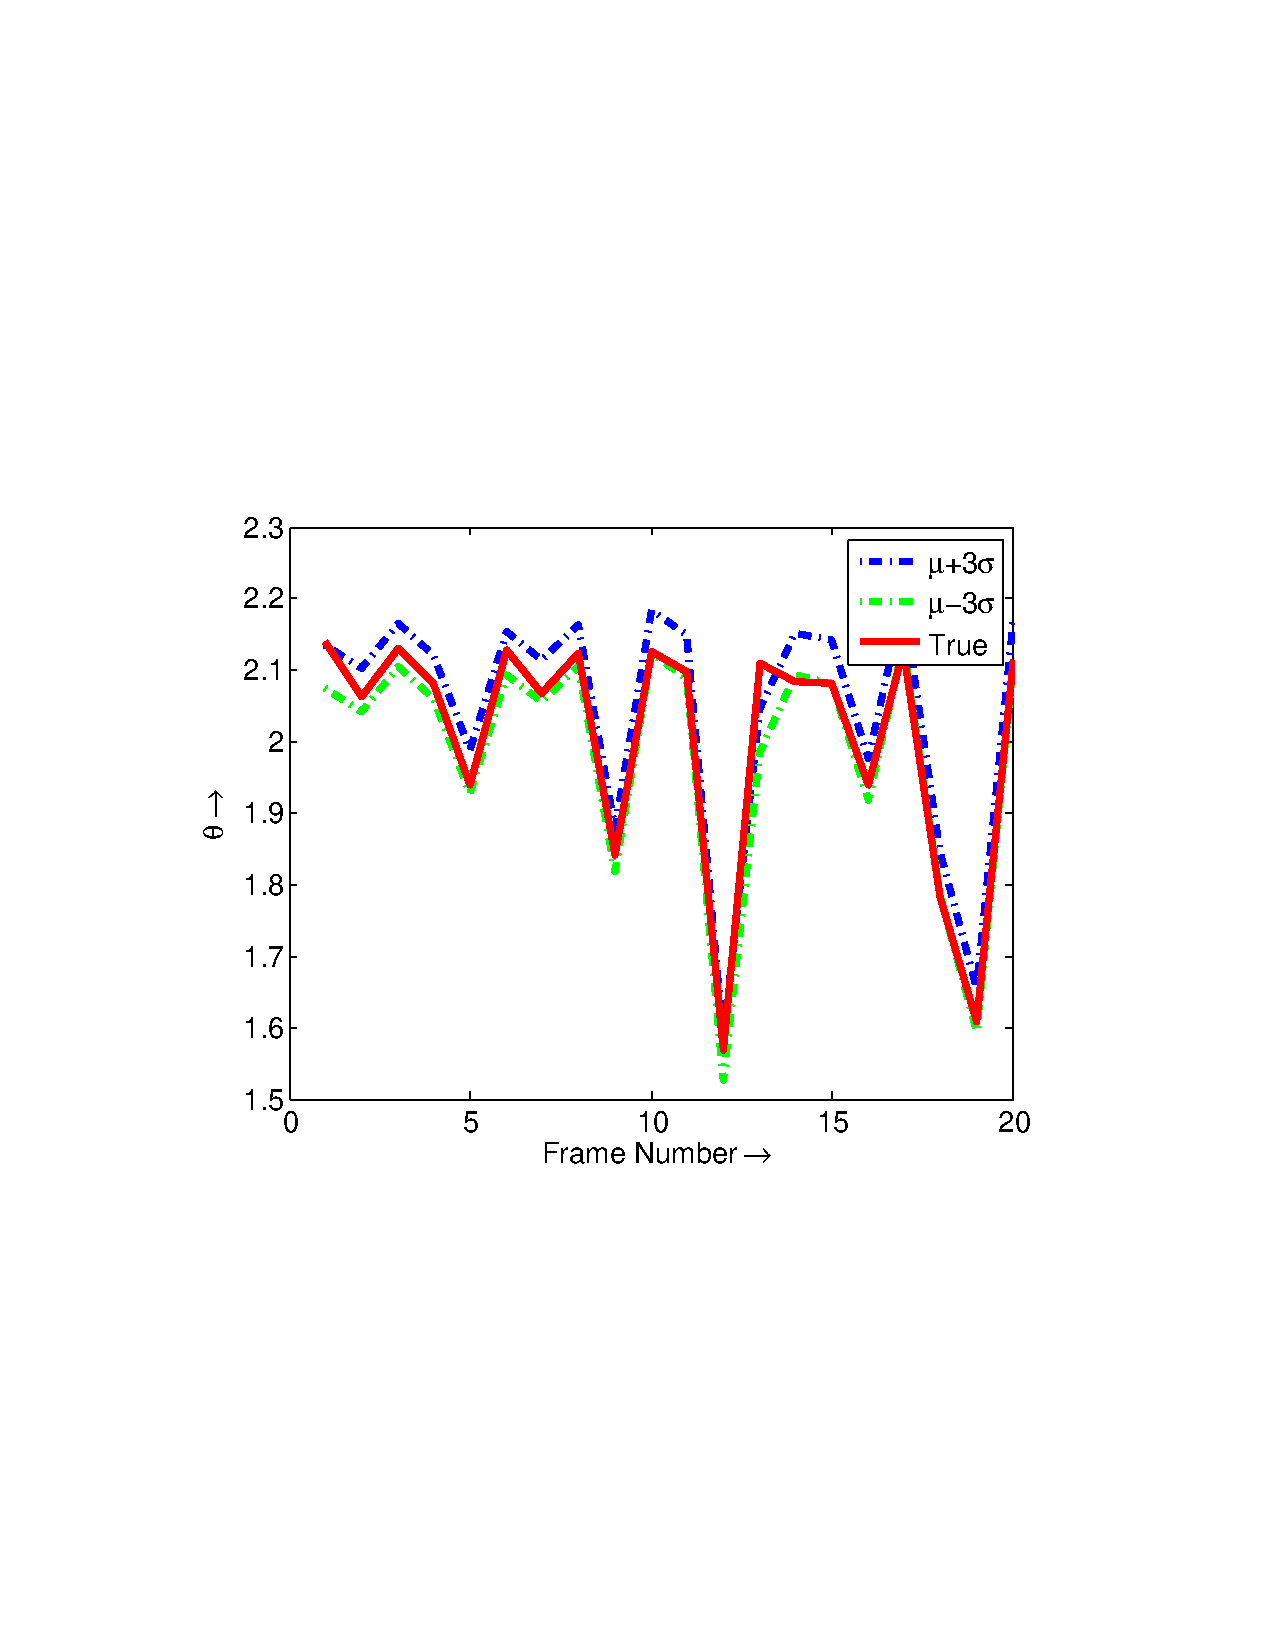
\includegraphics[width = 0.5\linewidth,trim= 20mm 80mm 35mm 85mm,clip]{figures/surgical/gaussian_estimation_1}
\caption{Gaussian Process regression with 3 sigma bounds plotted with true value of tool opening angle}\label{fig:three_sigma}
\end{figure}
\end{frame}

\begin{frame}{Visual Features}
\begin{block}{Ideal Features}
Unique, Invariant, Computationally Efficient
\end{block}
Histograms of Oriented Gradients (HOG) and Local Binary Patterns (LBP)
\begin{figure}
\centering
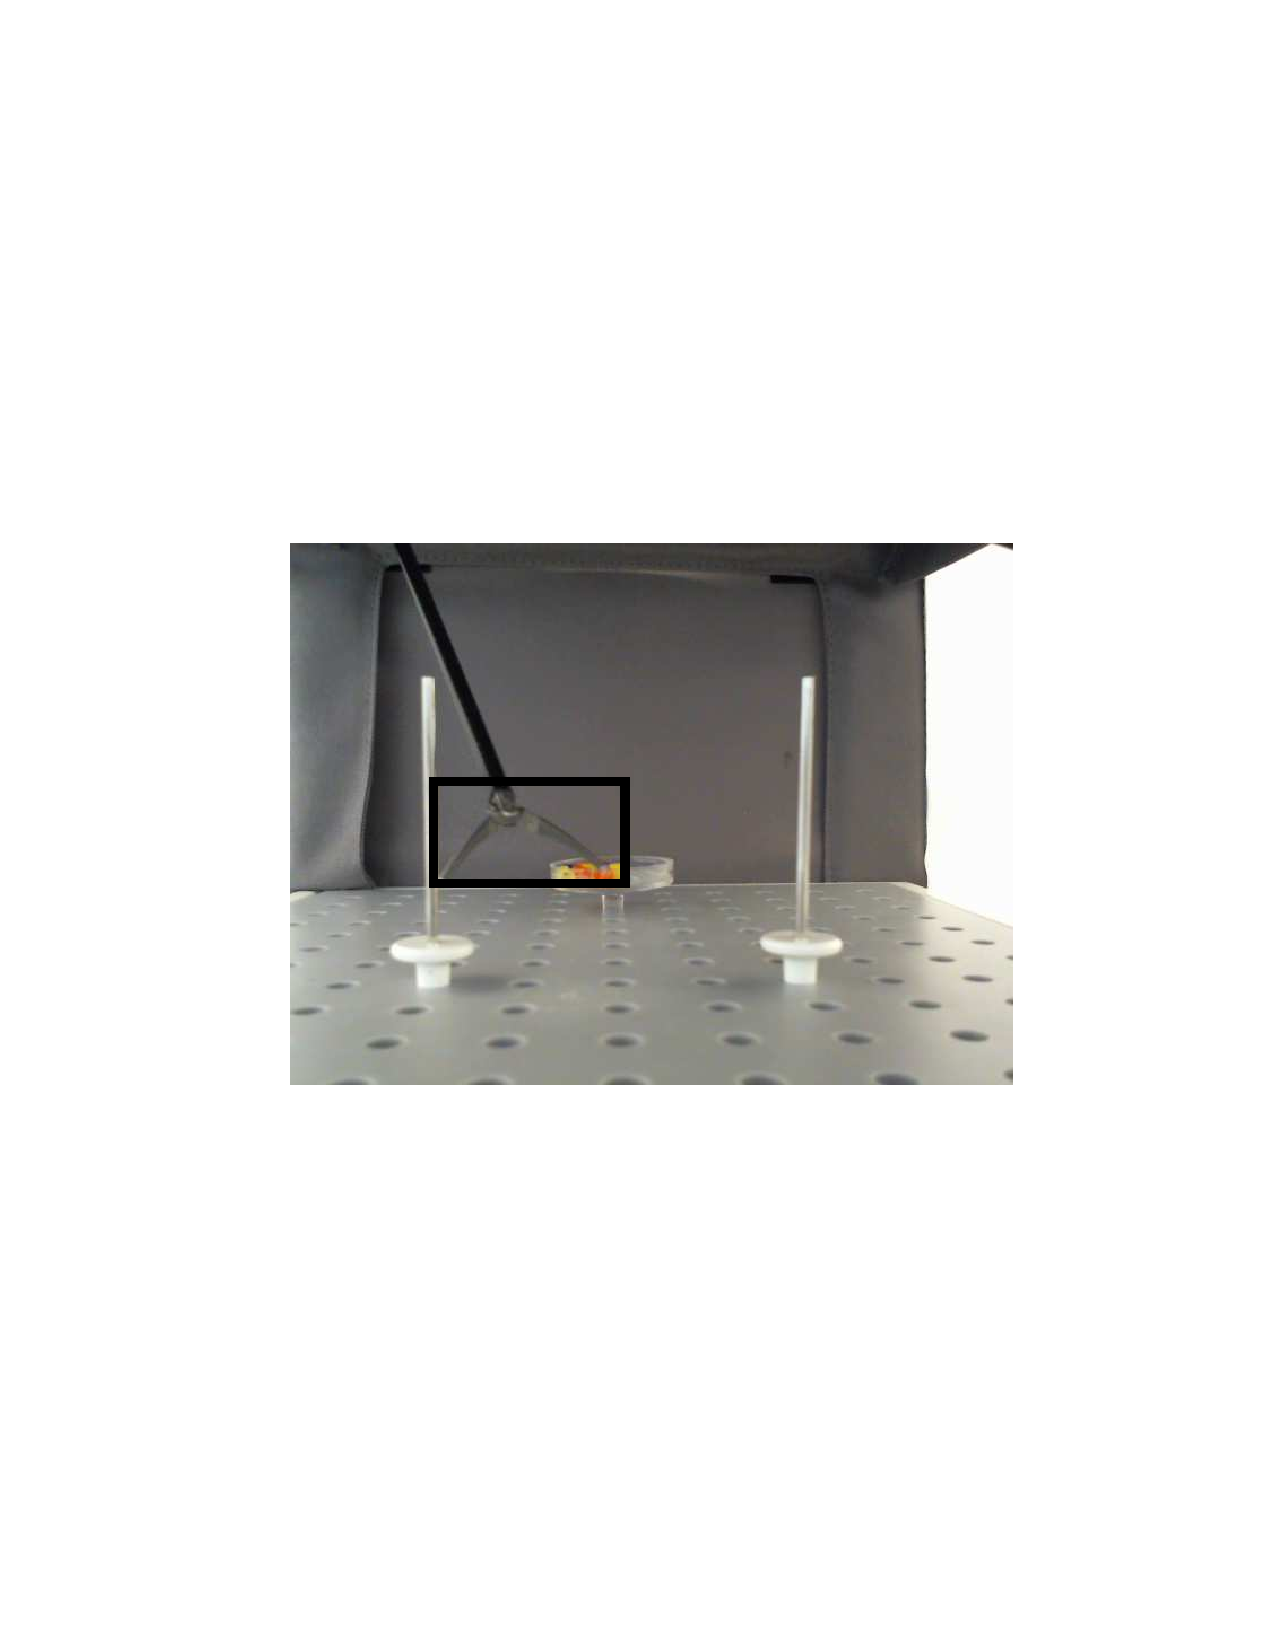
\includegraphics[width=0.45\linewidth,trim=40mm 106mm 80mm 100mm,clip]{figures/surgical/feature_pic}
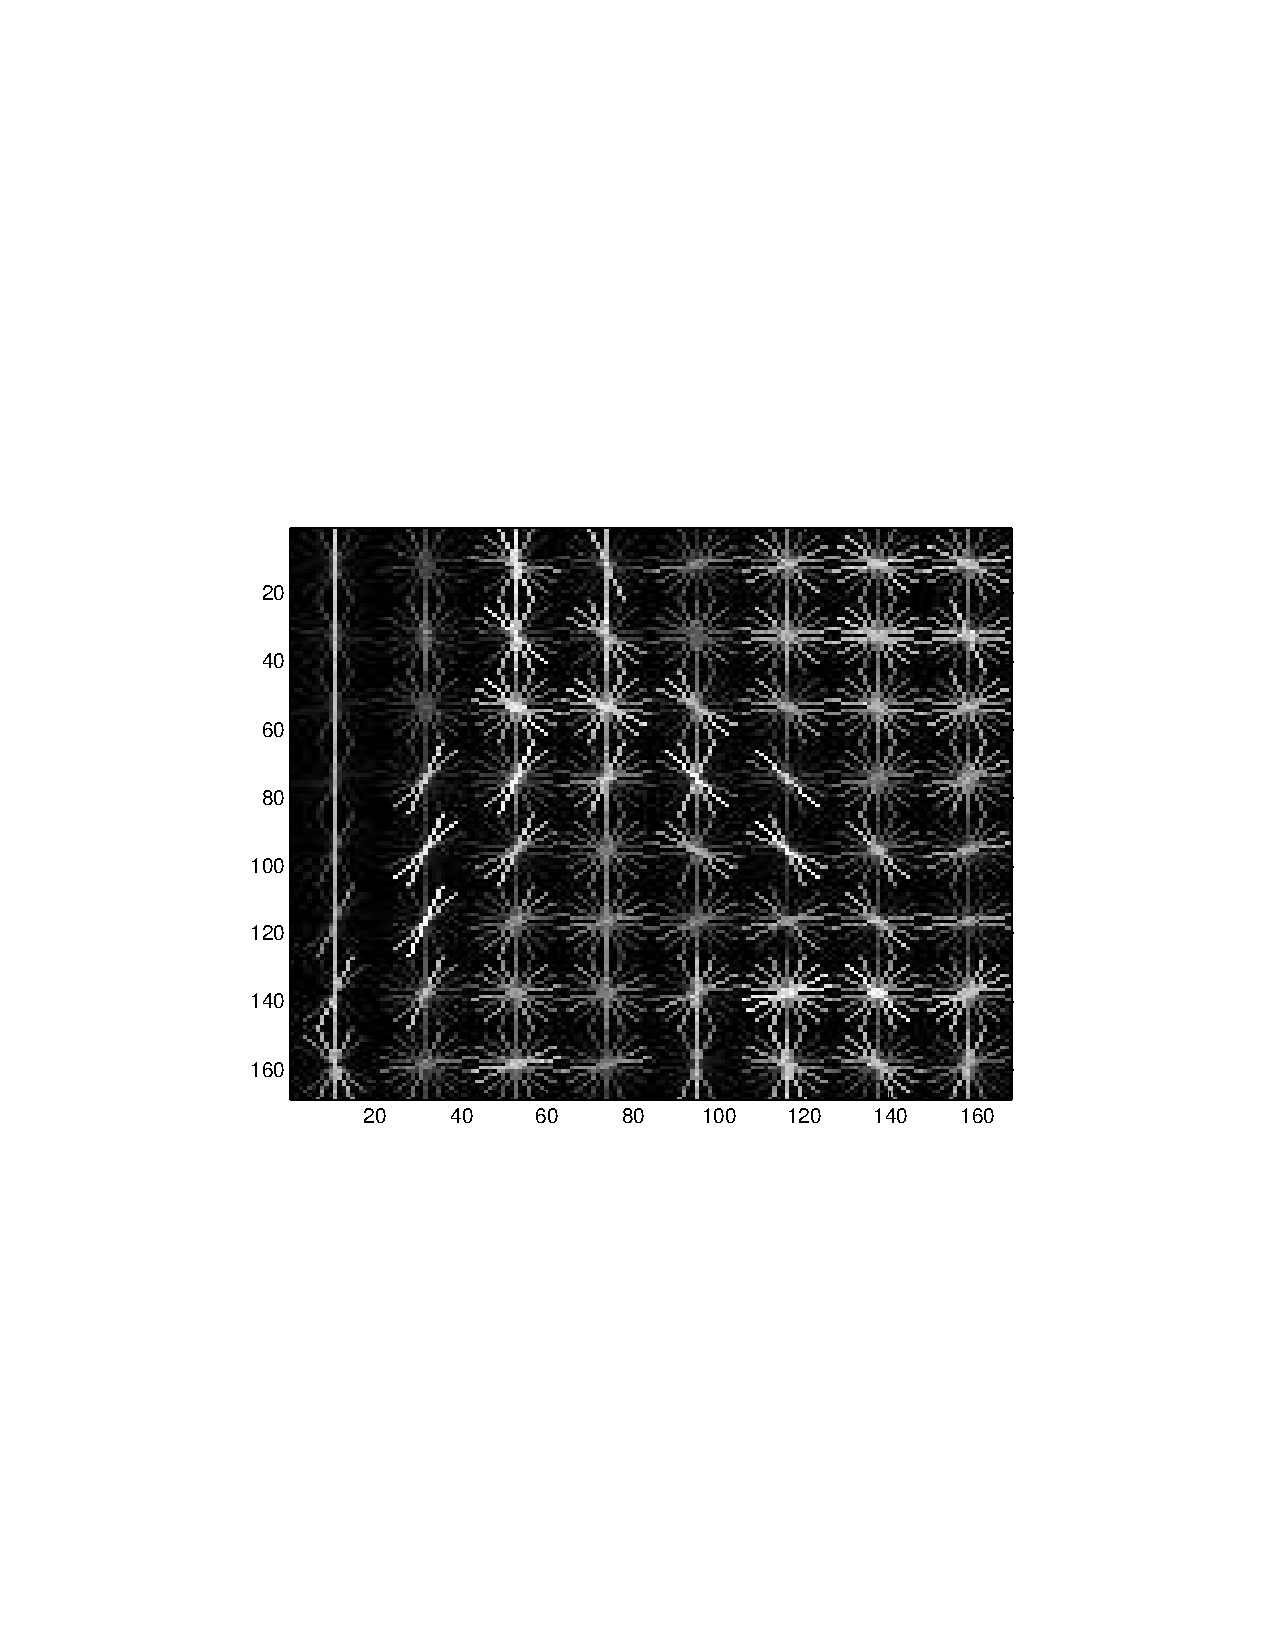
\includegraphics[width=0.45\linewidth,trim=50mm 93mm 40mm 70mm,clip]{figures/surgical/feature_pic_hog}
\caption{An example image with tool and corresponding HOG feature} \label{fig:hog}
\end{figure}
\end{frame}

\subsection[]{Experiments}
\begin{frame}{Experimental Data}
\begin{itemize}
\item Both moving and fixed part of a tool are tracked at $50$ fps
\item Endoscopic camera : $640 \times 480$ pixels at $15$ fps 
\item Entire dataset has $4346$ different tool poses
\item Sensing Noise: Motion blur, partial occlusions, lighting variation
\end{itemize}
\begin{figure}[h]
\centering
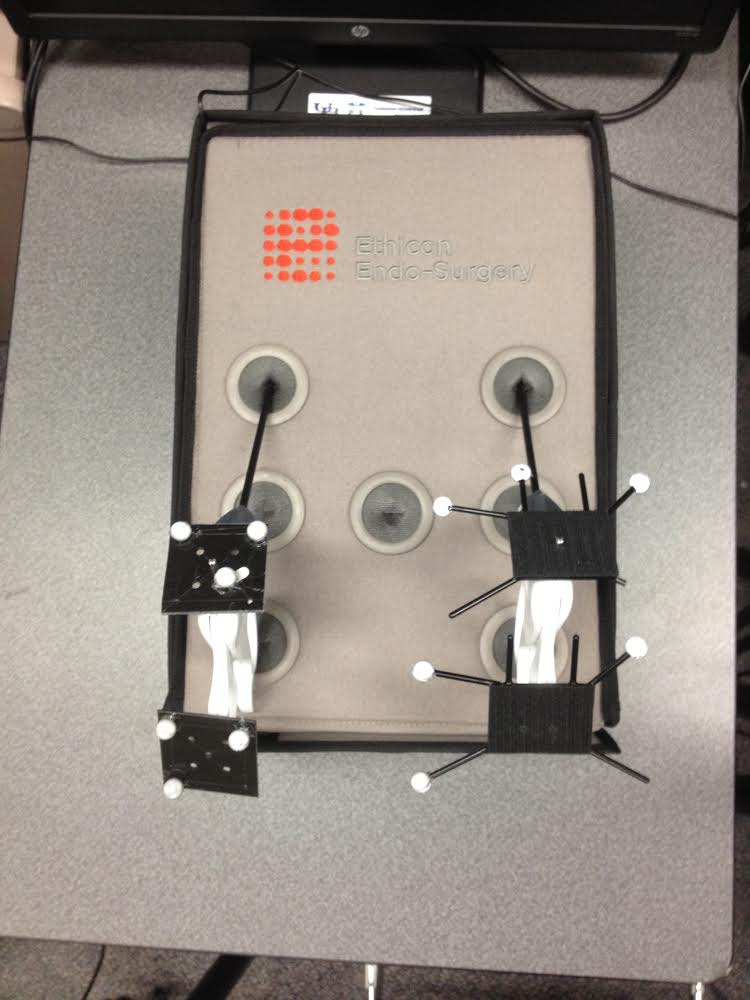
\includegraphics[height=0.4\columnwidth,trim= 40mm 50mm 30mm 35mm,clip]{figures/surgical/box}
\caption{Customized Box Trainer Setup Retrofitted with Optical Reflective Markers}
\label{fig:boxTrainer}
\end{figure}
\end{frame}

\begin{frame}{Results}
\begin{table}
\begin{tabular}{| c| c| c| }\hline
 Features &  Orientation Error & Opening Angle \\ \hline
HOG& 2.42  & 2.49\\ \hline
  LBP & 1.92 & 2.48\\ \hline
\end{tabular}
\caption{Tool pose estimate angular accuracy in degrees using different visual features}
\end{table}

\begin{figure}
\centering
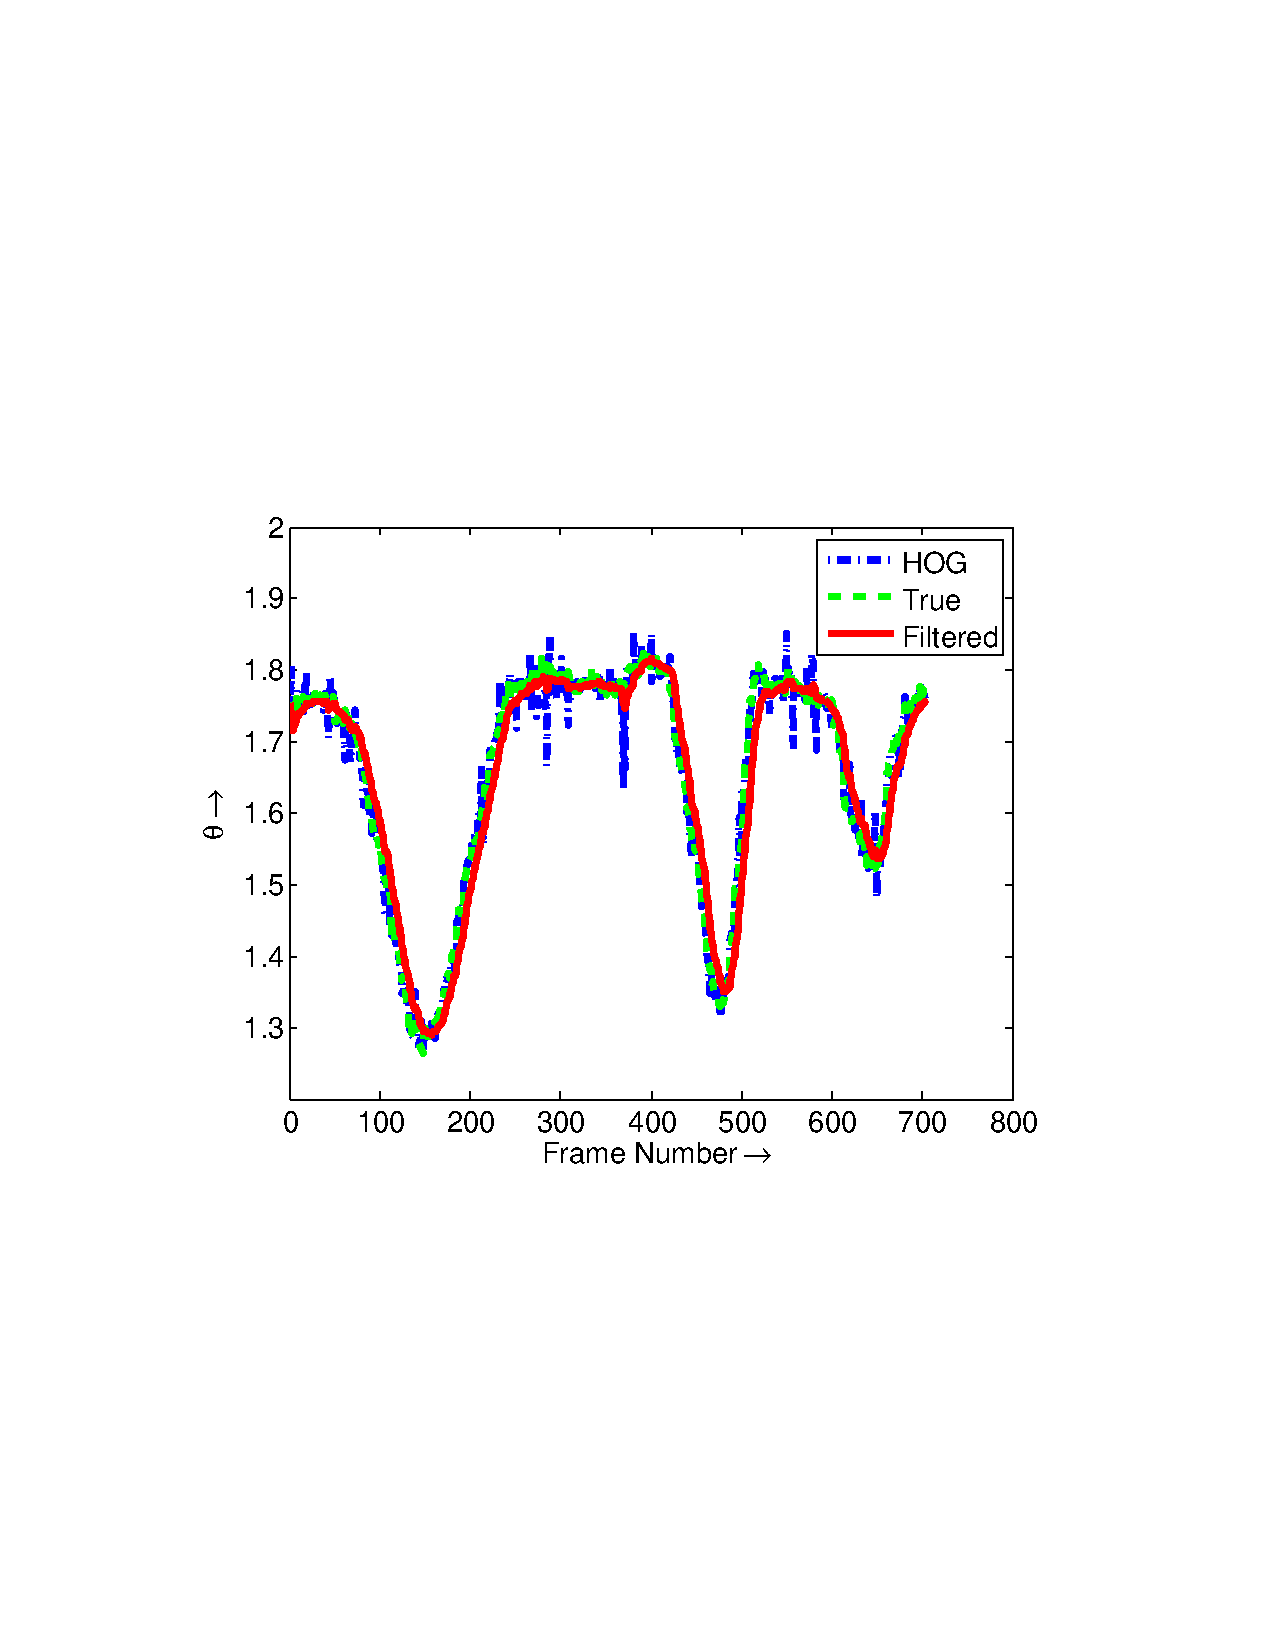
\includegraphics[width = 0.5\columnwidth,trim = 20mm 80mm 40mm 80mm,clip]{figures/surgical/kalman_filter}
\caption{True, Regression mean estimate and filtered estimates for tool opening angle} \label{fig:kalman_filter}
\end{figure}

\end{frame}

\begin{frame}{Visual Results}
\begin{figure}
\centering
\subfloat{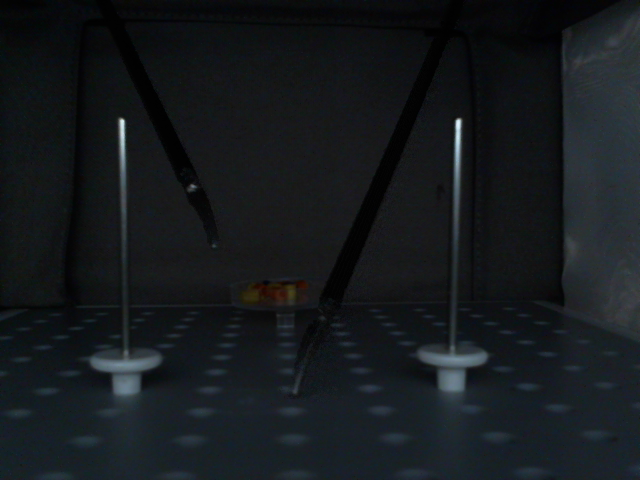
\includegraphics[width = 0.2\linewidth,trim = 32mm 10mm 70mm 30mm,clip]{figures/dark_ims/23_16_20_128}}
\subfloat{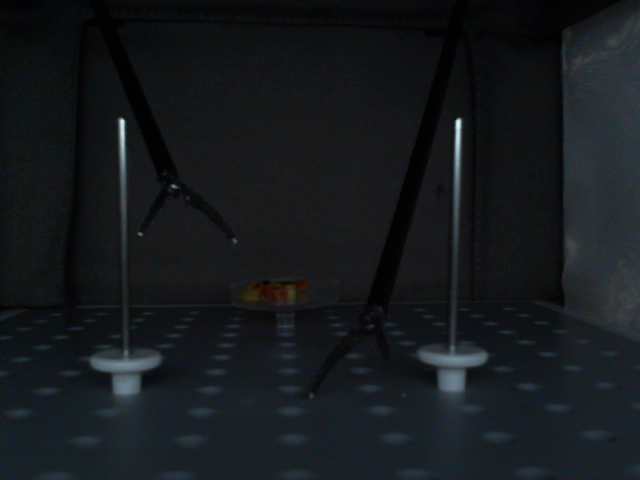
\includegraphics[width = 0.2\linewidth,trim = 32mm 10mm 70mm 30mm,clip]{figures/dark_ims/23_16_25_966}}
\subfloat{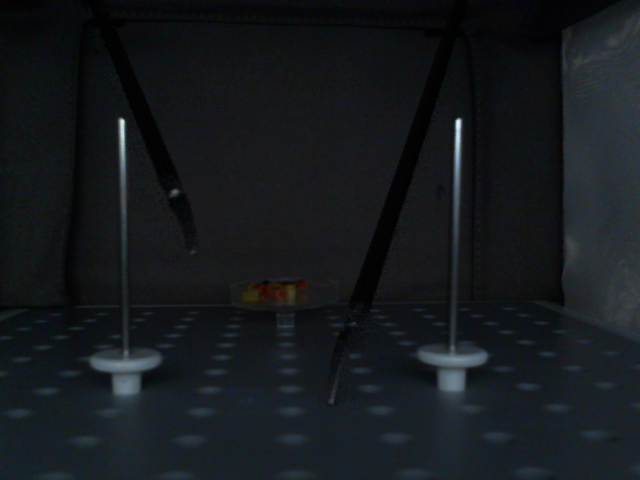
\includegraphics[width = 0.2\linewidth,trim = 32mm 10mm 70mm 30mm,clip]{figures/dark_ims/23_16_30_623}}
\subfloat{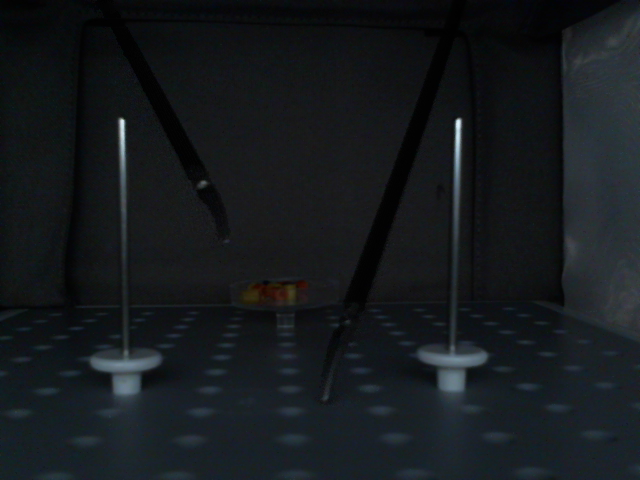
\includegraphics[width = 0.2\linewidth,trim = 32mm 10mm 70mm 30mm,clip]{figures/dark_ims/23_16_31_151}}
\subfloat{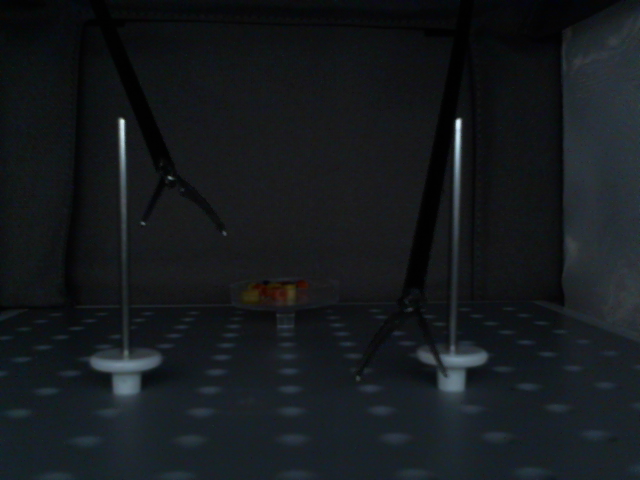
\includegraphics[width = 0.2\linewidth,trim = 32mm 10mm 70mm 30mm,clip]{figures/dark_ims/23_16_37_728}}\\
\vspace{-10pt}
\subfloat{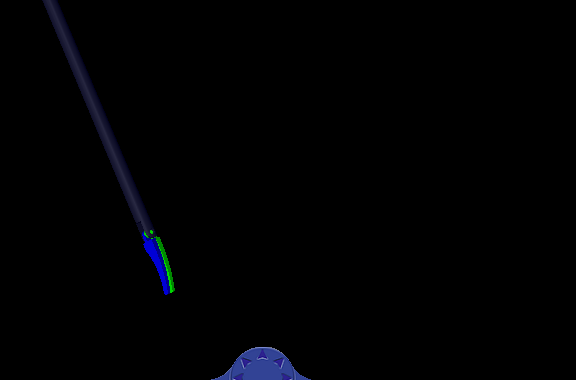
\includegraphics[width = 0.20\linewidth,trim = 32mm 15mm 102mm 30mm,clip]{figures/vr/scale_gt_dark_lbp_left/frame_52}}
\subfloat{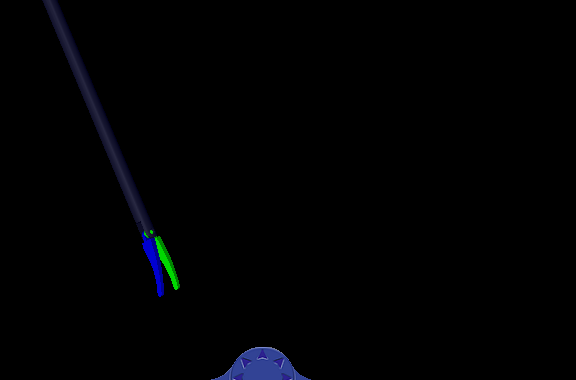
\includegraphics[width = 0.20\linewidth,trim = 32mm 15mm 102mm 30mm,clip]{figures/vr/scale_gt_dark_lbp_left/frame_139}}
\subfloat{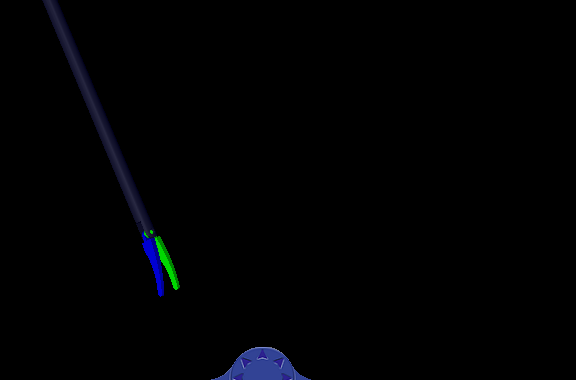
\includegraphics[width = 0.20\linewidth,trim = 32mm 15mm 102mm 30mm,clip]{figures/vr/scale_gt_dark_lbp_left/frame_209}}
\subfloat{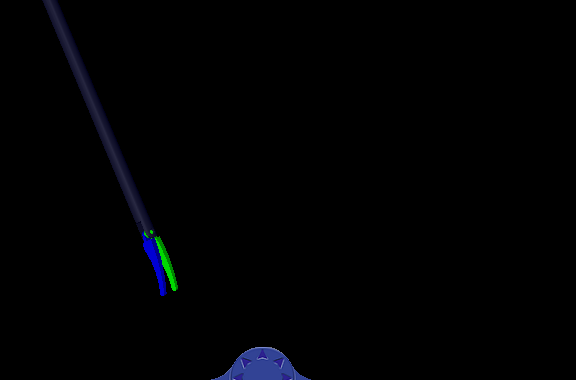
\includegraphics[width = 0.20\linewidth,trim = 32mm 15mm 102mm 30mm,clip]{figures/vr/scale_gt_dark_lbp_left/frame_217}}
\subfloat{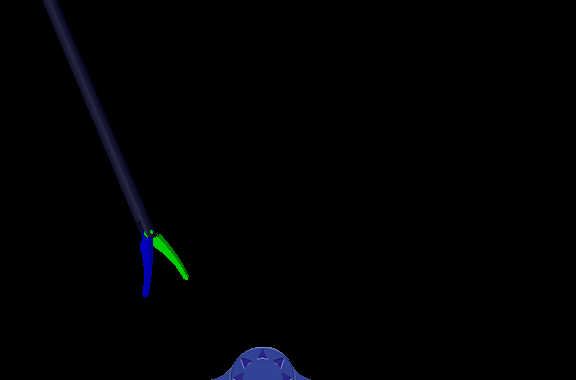
\includegraphics[width = 0.20\linewidth,trim = 32mm 15mm 102mm 30mm,clip]{figures/vr/scale_gt_dark_lbp_left/frame_285}}\\
\vspace{-10pt}
\subfloat{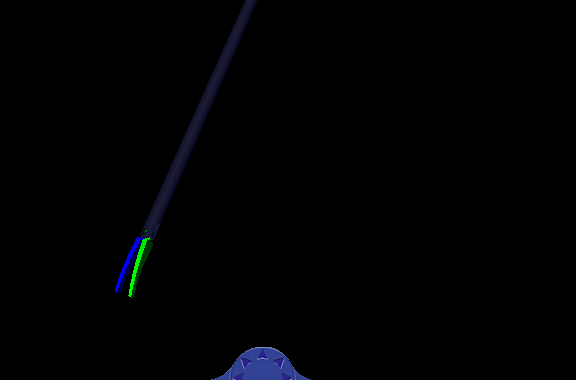
\includegraphics[width = 0.20\linewidth,trim = 32mm 15mm 102mm 30mm,clip]{figures/vr/scale_gt_dark_lbp_right/frame_52}}
\subfloat{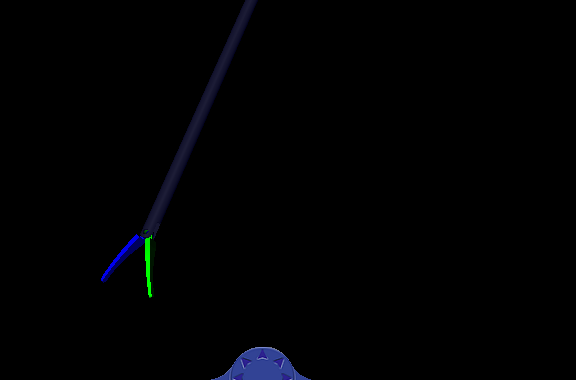
\includegraphics[width = 0.20\linewidth,trim = 32mm 15mm 102mm 30mm,clip]{figures/vr/scale_gt_dark_lbp_right/frame_139}}
\subfloat{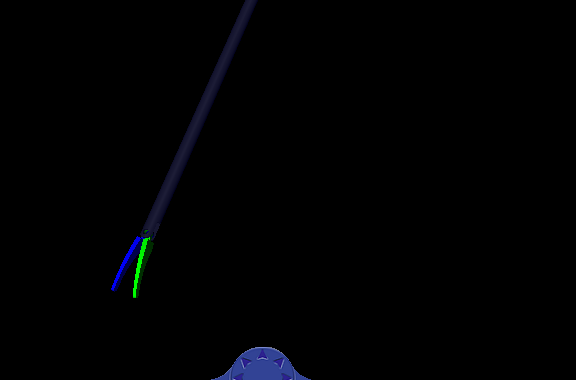
\includegraphics[width = 0.20\linewidth,trim = 32mm 15mm 102mm 30mm,clip]{figures/vr/scale_gt_dark_lbp_right/frame_209}}
\subfloat{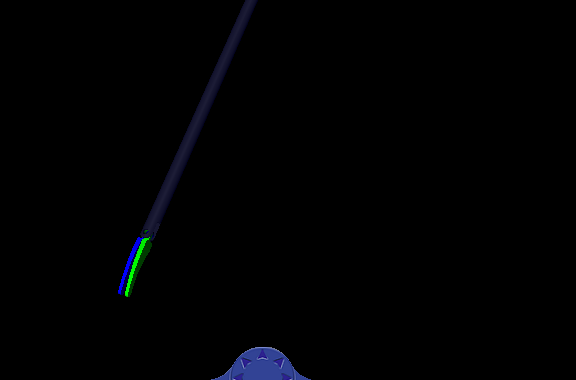
\includegraphics[width = 0.20\linewidth,trim = 32mm 15mm 102mm 30mm,clip]{figures/vr/scale_gt_dark_lbp_right/frame_217}}
\subfloat{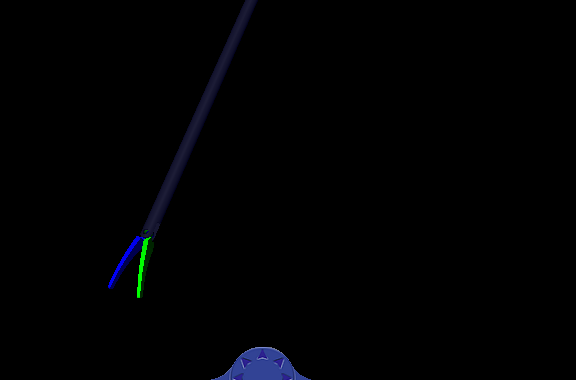
\includegraphics[width = 0.20\linewidth,trim = 32mm 15mm 102mm 30mm,clip]{figures/vr/scale_gt_dark_lbp_right/frame_285}}\\
%\caption{Representative video frames for a ``dark" sequence in the collected dataset obtained using GPR to estimate tool opening angle. First row shows the image frame, second row shows the orientation and opening angle of the left tool and the third row shows the orientation and opening angle of the right tool using LBP features.}
%\label{fig:dark_results_pose}
\end{figure}

\end{frame}

\begin{frame}{Conclusion}
\begin{itemize}
\item Real-time method to predict tool pose using generic visual features
%that are not specific to any tool and environment setting.
\item Robust variance estimates along with mean predictions
\item Variance estimate is demonstrated to be useful for filtering
\item Experimental results using a customized box trainer demonstrate good tool pose prediction 
\end{itemize}
\end{frame}

\begin{frame}{Publications}
\begin{block}{Journal}
\begin{enumerate}
\item \textbf{S. Kumar}, J. Sovizi, V. Krovi, ``Error Propagation on SE(3) for Surgical Tool Pose Filtering" (In Preparation)
\item P. Agarwal, \textbf{S. Kumar}, J. Ryde, J. Corso, and V. Krovi, ``Estimating Dynamics On-the-fly Using Monocular Video For Vision-Based Robotics", IEEE/ASME Transactions on Mechatronics, 2013.
\end{enumerate}
\end{block}

\begin{block}{Conference}
\begin{enumerate}
\item \textbf{S. Kumar}, J. Sovizi, M. S. Narayanan, V. Krovi, ``Surgical Tool Pose Estimation from Monocular Endoscopic Videos", IEEE International Conference on Robotics and Automation (ICRA), 2015
\item P. Agarwal, \textbf{S. Kumar}, J. Ryde, J. Corso, and V. Krovi,
``Estimating Human Dynamics On-the-fly Using Monocular Video for Pose
Estimation", Robotics: Science and Systems VIII, 2013
\end{enumerate}
\end{block}
\end{frame}





%Dynamic Map
%\include{dynamic_map}
% Toyota Project
%\include{toyota_project}

\begin{frame}[standout]
Questions?
\end{frame}
\end{document}
